%%%%%%%%%%%%%%%%%%%%%%%%%%%%%%%%%%%%%%%%%%%%%%%%%%%%%%%%%%%%%%%%%%%%%%%%
% Plantilla TFG/TFM
% Universidad de A Coruña. Facultad de Informática
% Realizado por: Welton Vieira dos Santos
% Modificado: Welton Vieira dos Santos
% Contacto: welton.dossantos@udc.es
%%%%%%%%%%%%%%%%%%%%%%%%%%%%%%%%%%%%%%%%%%%%%%%%%%%%%%%%%%%%%%%%%%%%%%%%


\chapter{Desarrollo Artístico}
\section{Antecedentes}
En el año 2500 la Tierra era un yermo vacío y la humanidad la abandonó, 
mandando robots autoconscientes steampunk a explorar el espacio, ahora vivían colonizando el espacio. Figura \ref{fig:TierraDevastada}.

\begin{figure}[H]
	\centering
	\includegraphics[scale=0.80]{imagenes/terraDevastada.png}
	\caption{\label{fig:TierraDevastada}Tierra devastada}
\end{figure}

\section{Ambientación}
La historia se transcurre en una enorme y antigua nave en la que suceden cosas extrañas, de la que nuestro protagonista tendrá que huir.
ISS Manticore (Figura \ref{fig:ISSManticore}) es la nave misteriosa donde nuestro protagonista tenía que entregar un paquete.  

\begin{figure}[H]
	\centering
	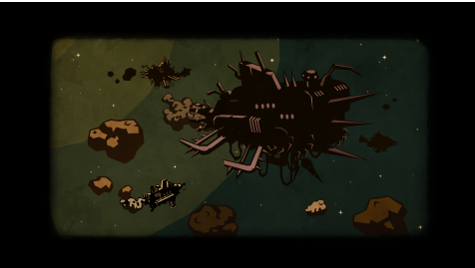
\includegraphics[scale=0.80]{imagenes/2.png}	
	\caption{\label{fig:ISSManticore}ISS Manticore}
\end{figure}

\section{Historia}
Jackie (Figura \ref{fig:Jackie})es un cartero espacial que tiene que entregar un paquete en una misteriosa nave, pero cuando llega no hay nadie, y acaba encerrado en la misteriosa nave de la que tendrá que escapar. Cuando nuestro protagonista abre el paquete, verá que es un arma de fuego, la tendrá que usar para abrirse paso a través de la nave contra los misteriosos moradores que se vaya encontrando en ella.

\section{Personajes}
\begin{itemize}
	\item \textbf{Jackie:} Nuestro protagonista, no tiene muchas luces, pero sabe sobrevivir
	\begin{figure}[H]
		\centering
		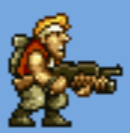
\includegraphics[scale=0.95]{imagenes/personaje_1.png}	
		\caption{\label{fig:Jackie} Aspecto de Jackie}
	\end{figure}
	\item \textbf{Enemigos:} En esta enorme nave habitan unos seres que al parecer no les gusta mucho la compañía de otros, por lo que te atacaran si te cruzas en su camino.
	\item \textbf{Octopus:} Son unos seres extraños fruto de un experimento de crear inteligencia artificial utilizando cerebros biológicos. 
	\begin{figure}[H]
		\centering
		
\includegraphics[scale=0.95]{imagenes/octopus.png}	
		\caption{\label{fig:Octopus}Aspecto de un Octopus}
	\end{figure}
	\item \textbf{Tortuga:} Alguien se olvidó de alimentar a las mascotas de la nave, pero por alguna razón se siguen moviendo,y parecen hambrientas. 
	\begin{figure}[H]
		\centering
		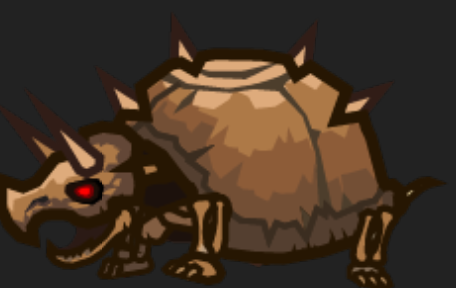
\includegraphics[scale=0.60]{imagenes/tortuga.png}	
		\caption{\label{fig:Tortuga}Aspecto de una Tortuga}
	\end{figure}
	\newpage
	\item \textbf{Spiderbots:} Alguien que se aburría en esta nave se le ocurrió la brillante idea de ponerle patas a las torretas, y parece que muy bien no salió. 
	\begin{figure}[H]
		\centering
		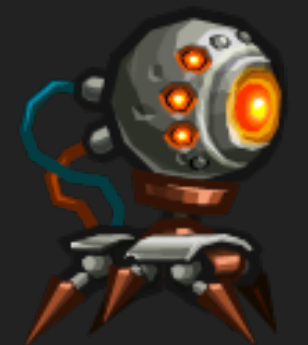
\includegraphics[scale=0.6]{imagenes/spiderbot.png}	
		\caption{\label{fig:Spiderbots}Aspecto de un Spiderbot}
	\end{figure}
\end{itemize}

\section{Jugabilidad}
Side scroller en el que completas niveles estilo metroidvania, en el que el 
personaje pelea:  
\begin{itemize}
	\item Utilizando un arma de fuego (escopeta - Figura \ref{fig:escopeta}),
	 en el que avanzamos de forma similar a juegos como “My Friend Pedro”
	   avanzando por diferentes niveles acabando con los enemigos(Figura 1.6),
	    con una estética de enemigos y de ambientación ligeramente steampunk.
\end{itemize}
\begin{figure}[H]
	\centering
	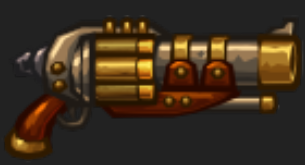
\includegraphics[scale=0.80]{imagenes/escopeta.png}	
	\caption{\label{fig:escopeta}Ejemplo de la escopeta}
\end{figure}

\begin{figure}[H]
	\centering
	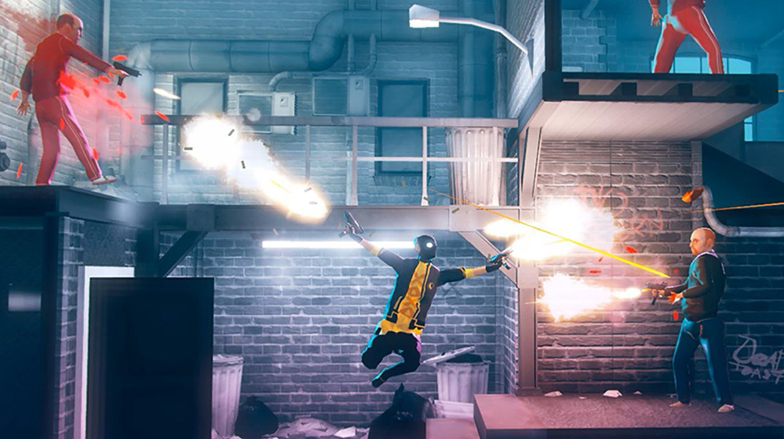
\includegraphics[scale=0.45]{imagenes/5.png}	
	\caption{\label{fig:ambiente}Ejemplo de un posible escenario y la dinámica de disparos en tempo real}
\end{figure}

\section{Items para el personaje}
\begin{itemize}
	\item \textbf{Vidas:}.Para recuperar vida y ayudar al jugador e incentivarlo a explorar el escenario.(Figura \ref{fig:Ejemplo Vida})
	\begin{figure}[H]
		\centering
    	
\includegraphics[scale=0.95]{imagenes/vida.png}	
		\caption{\label{fig:Ejemplo Vida}Imagen de item para recuperar a vida}
	\end{figure}
	\item \textbf{Wrench:} Items coleccionables necesarios para completar
			el segundo nivel en el que tienes que recoger piezas para reparar el motor de la nave y así también hacer al jugador explorar el escenario (Figura \ref{fig:Wrench}).
	\begin{figure}[H]
		\centering
		
\includegraphics[scale=0.55]{imagenes/wrench.png}	
		\caption{\label{fig:Wrench}Imagen de wrench representada por una llave inglesa girando}
	\end{figure}
\end{itemize}

\section{Lugares}
\subsection{ISS Manticore}
La nave en la que se desarrolla el juego, está llena de misterios y seres extraños poco amistosos
tiene diferentes zonas y salas dentro,
en este juego se incluyen 3 salas, que corresponderían a 3 niveles.

\subsection{Sala de calderas de la nave}
El primer lugar al que llega el protagonista, en esta zona de la nave se encuentran todo el sistema del motor de la nave.

\subsection{Bodega de carga}
Es la bodega de carga de la nave, donde está el almacen y tiene un montón de extraños trastos viejos de la nave y muchas herramientas que serán de utilidad al protagonista.

\subsection{Puente de mando}
La última sala que el protagonista deberá atravesar, y así conseguir al fin huir de la nave.

\section{Guion}
\subsection{Fase 1 - Sala de calderas}
La escena empieza con el cartero intentando entregar ese supuesto paquete a la nave y al llegar cerca de la nave el personaje \textbf{Jackie} se da cuenta que en esa nave no hay nadie que pueda responder y el toma la decisión de entrar en la nave y el mismo se queda atrapado. 

Para salir de esa nave el tiene que buscar otra salida. Jackie decide abrir el paquete y se dentro del mismo se encuentra un arma y decide seguir hacia delante para intentar localizar otra salida.

\subsection{Fase 2 - Almacen}
Esa escena empezará con unos de los enemigos dañando un motor de la sala de calderas lo que obriga a nuestro personaje (Jackie) a intentar localizar piezas para reparar ese motor dañado avanzando a este siguien escenario que será el almacen de la bodega de carga.
Nuestro personaje encuentra herramientas y piezas al 
recorrer el camino que pueden ser utilizadas para reparar el motor.
Además de ir derrotando los enemigos que van apareciendo a medida que Jackie avanza.
Para terminar la fase, Jackie tiene que haber recogido todas las piezas que se encuentra en esa fase para reparar el motor.

\subsection{Fase 3 - Casco superior de nave}

Esa fase se empieza una batalla final con los últimos enemigos que protejen la mesa de mando donde nuestro personaje tiene que enchufar una tarjeta, que contiene un chip que permite Jackie efetuar un pedido de auxilio. Al momento que Jackie enchufa la tarjeta, la nave sufre un apagon debido daños causados anteriormente por los enemigos.

\section{Videojuego en 3D}

\subsection{Fases}
\subsubsection{Fase 1 - Motores exteriores de la nave}
Nuestro protagonista, tiene que salir a arreglar el motor de la nave para recuperar la electricidad y
 que se envíe la llamada de ayuda, así que tendrá que salir fuera de la nave (por lo que no hay gravedad) ,
  y con su pistola gancho tendrá que ir avanzando por la turbinas girando y demás elementos flotando
   hasta llegar al motor a arreglar 

\subsubsection{Fase 2 - Zonas de motores}
El protagonista se tiene que defender de enemigos mientras repara el motor.

\subsubsection{Fase 3 - Espacio exterior}
Una nave para salvarle aparece, nuestro protagonista tendrá que ir escalando entre basura espacial y cajas
(de la sala de carga) flotando en el espacio entre las dos naves para poder huir y alcanzar a la otra nave.
(las torretas de la nave de la que huye le pueden ir disparando mientras para que no huya).
